\documentclass[aspectratio=169,11pt]{beamer}
\usetheme[progressbar=frametitle,numbering=fraction]{metropolis}
\usepackage[T1]{fontenc}
\usepackage[utf8]{inputenc}
\usepackage[portuguese]{babel}
\usepackage{amsmath,amssymb}
\usepackage{booktabs}
\usepackage{siunitx}
\usepackage{graphicx}
\usepackage{tikz}
\graphicspath{{figures/}}

\newcommand{\U}{\boldsymbol{U}}
\newcommand{\p}{\boldsymbol{p}}
\newcommand{\q}{\boldsymbol{q}}
\newcommand{\rr}{\boldsymbol{r}}
\newcommand{\nota}[1]{{\scriptsize\color{gray}#1}}
% linhas de tabela geradas por scripts/deck_figs.py: \@@input e expansivel,
% entao funciona dentro de tabular (\input nao funciona antes de \midrule)
\makeatletter\newcommand{\inputrows}[1]{\@@input #1 }\makeatother

\title{Problema inverso do ECG: o Método 1}
\subtitle{Fontes em $S$, solve blindado e $\Delta$-Poisson}
\author{Yan B. Werneck}
\date{Outubro de 2026}

\begin{document}

\maketitle

\begin{frame}{Roteiro}
  \tableofcontents
\end{frame}

% Parte 1: o operador Delta-PoIssoNN, como na abertura de 2026-10_progresso
% (sections/01_operador.tex; equacoes e numeracao de "Problemas no Operador").

\section{O operador $\Delta$-PoIssoNN}

\begin{frame}{O operador $\Delta$-PoIssoNN}
  \small
  \renewcommand{\arraystretch}{2.4}
  \begin{columns}[T,totalwidth=1.05\textwidth]
    \begin{column}{0.51\textwidth}
      \textbf{Definição}\\[-0.4em]
      \begin{tabular}{@{}l@{\hspace{0.35em}}r@{\;}l@{\hspace{0.5em}}l@{}}
        \nota{(1)} & $\|\U\nabla\varphi\|$ & $= 1$ & \nota{Eikonal anisotrópica}\\
        \nota{(2)} & $\p$ & $:= \dfrac{\nabla\varphi}{\|\nabla\varphi\|}$ & \nota{gradiente unitário}\\
        \nota{(3)} & $\nabla\varphi$ & $= \dfrac{\p}{\|\U\p\|}$ & \nota{da Eikonal e (2)}\\
        \nota{(4)} & $\Delta\varphi$ & $= \nabla\cdot\left(\dfrac{\p}{\|\U\p\|}\right)$ & \nota{divergente de (3)}\\
        \nota{(5)} & $\p(\boldsymbol{x})$ & $:= \mathrm{NN}\bigl(v(\boldsymbol{x});\boldsymbol{\theta}\bigr)$ & \nota{a rede}
      \end{tabular}
    \end{column}
    \begin{column}{0.53\textwidth}
      \textbf{O operador:} (5) em (3)\\[-0.4em]
      \begin{tabular}{@{}l@{\hspace{0.35em}}r@{\;}l@{\hspace{0.5em}}l@{}}
        \nota{(6)} & $\nabla\varphi$ & $= \dfrac{\mathrm{NN}(v;\boldsymbol{\theta})}{\|\U\,\mathrm{NN}(v;\boldsymbol{\theta})\|}$ & \nota{(5) em (3)}\\
        \nota{(7)} & $\Delta\varphi$ & $= \nabla\cdot\left[\dfrac{\mathrm{NN}(v;\boldsymbol{\theta})}{\|\U\,\mathrm{NN}(v;\boldsymbol{\theta})\|}\right]$ & \nota{divergente de (6)}\\
        \nota{(8)} & $\Delta\varphi$ & $= f$ & \nota{$f$ pelo FEM}\\
        \nota{(9)} & $K\boldsymbol{\varphi}$ & $= \boldsymbol{b}$ & \nota{Poisson, FEM}\\
        \nota{(10)} & $\varphi$ & $\leftarrow \varphi - \min\varphi$ & \nota{remove a constante}
      \end{tabular}
    \end{column}
  \end{columns}
\end{frame}

\begin{frame}{Por que o operador não é exato}
  \small
  Seja $\q := \p/\|\U\p\|$ \nota{(11)}. Para que $\p$ venha de um mapa de
  ativação é preciso $\q = \nabla\varphi$, e portanto
  \[
    \nabla\times\left(\frac{\p}{\|\U\p\|}\right) = \boldsymbol{0}
    \qquad\text{\nota{(17), integrabilidade}}
  \]
  O Poisson usa só $\nabla\cdot\q$: devolve um $\varphi$ mesmo com
      $\nabla\times\q \neq \boldsymbol{0}$.
  \vfill
  {\scriptsize\color{gray} Demonstração Overleaf de 20/09.}
\end{frame}

% Parte 2: o Metodo 1, no mesmo estilo do operador.
% Fonte: nota do screened Poisson (02/10/2026, reports/investigating_v2/
% yan_screened_poisson_plan.pdf), Secs. 3-6.2 e 8; codigo
% core/screened.py, core/screened_front.py (ScreenedFront).
% Numeracao continua depois de (17).

\section{O Método 1}

\begin{frame}{O Método 1: fontes em $S$, screened Poisson, $\Delta$-Poisson}
  \small
  \renewcommand{\arraystretch}{2.5}
  \textbf{Definição}\\[-0.4em]
  \begin{tabular}{@{}l@{\hspace{0.6em}}r@{\;}l@{\hspace{1.4em}}l@{}}
    \nota{(18)} & $g(\boldsymbol{s})$ & $:= \mathrm{NN}\bigl(v(\boldsymbol{s});\boldsymbol{\theta}\bigr), \quad \boldsymbol{s}\in S$ & \nota{tempo de cada candidato em $S$}\\
    \nota{(19)} & $w(\boldsymbol{s})$ & $= \exp\!\left(-\dfrac{g(\boldsymbol{s}) - \min_S g}{\varepsilon}\right)$ & \nota{peso de cada fonte}\\
    \nota{(20)} & $u - \varepsilon^2\,\nabla\cdot(A\nabla u)$ & $= B_S\,w, \quad A = \U^{T}\U$ & \nota{screened Poisson}\\
    \nota{(21)} & $\q_g$ & $= -\dfrac{\nabla u}{\|\U\nabla u\|}$ & \nota{direção, no lugar de (11)}\\
    \nota{(22)} & $\Delta\varphi$ & $= \nabla\cdot\q_g$ & \nota{o operador, (8)--(10)}
  \end{tabular}
\end{frame}

\begin{frame}{O Método 1 no FEM}
  \small
  \renewcommand{\arraystretch}{2.5}
  \textbf{Discretização}\\[-0.4em]
  \begin{tabular}{@{}l@{\hspace{0.6em}}r@{\;}l@{\hspace{1.4em}}l@{}}
    \nota{(23)} & $H_\varepsilon$ & $= M + \varepsilon^2 K_A$ & \nota{$M$: lumped mass; $K_A$: rigidez com $A$}\\
    \nota{(24)} & $(\boldsymbol{b}_S)_s$ & $= a_s\, w_s, \quad s \in S$ & \nota{$a_s$: área de superfície do nó $s$}\\
    \nota{(25)} & $H_\varepsilon\,\boldsymbol{u}$ & $= \boldsymbol{b}_S$ & \nota{SPD, sem constante livre}\\
    \nota{(26)} & $\q_g$ & $=$ (21) em cada elemento, média nos nós & \nota{como $\p$ no Método 0}\\
    \nota{(27)} & $K\boldsymbol{\varphi}$ & $= \boldsymbol{b}(\q_g), \quad \varphi \leftarrow \varphi - \min\varphi$ & \nota{(9)--(10), sem mudança}
  \end{tabular}
\end{frame}

\begin{frame}{Por que $-\varepsilon\log u$ é um tempo}
  \small
  Longe de $S$, com $\psi = -\varepsilon\log u$, a equação (20) vira
  \[
    \nabla\psi^{T}\!A\,\nabla\psi \;-\; \varepsilon\,\nabla\cdot(A\nabla\psi) \;=\; 1
    \qquad\text{\nota{Eikonal viscosa; $\varepsilon \to 0$ dá (1)}}
  \]
  Com a função de Green do screened Poisson, $G_\varepsilon(\boldsymbol{x},\boldsymbol{s}) \approx C_\varepsilon\, e^{-T(\boldsymbol{s},\boldsymbol{x})/\varepsilon}$:
  \[
    -\varepsilon\log u(\boldsymbol{x}) \approx \operatorname*{softmin}_{\boldsymbol{s}\in S}\,
      \bigl[g(\boldsymbol{s}) + T(\boldsymbol{s},\boldsymbol{x})\bigr]
  \]
  \vspace{-0.6em}
  \begin{itemize}\setlength{\itemsep}{0.1em}\footnotesize
    \item cada candidato entra com o seu tempo $g(\boldsymbol{s})$, sem resolver a Eikonal;
    \item só tempos relativos contam: $g + C$ multiplica $u$ por $e^{-C/\varepsilon}$;
    \item as fontes ficam em $S$ por construção, sem termo $L_S$;
    \item $\nabla\times\q_g = \boldsymbol{0}$ não é garantido (normalização anisotrópica): o $\Delta$-Poisson continua necessário.
  \end{itemize}
  \vspace{-0.3em}
  {\scriptsize\color{gray} Nos resultados: $\varepsilon = 2$ ms, lumped mass, $H_\varepsilon$ fatorado uma vez com as velocidades fixas.}
\end{frame}

% Custo: problems/purkinje_roots/scripts/bench_mesh.py (.114, RTX 4070 Ti
% SUPER, 2026-10-08), via reports/investigating_v2/handoff_camps_papers.md.
\begin{frame}{Método 0 e Método 1}
  \small
  \renewcommand{\arraystretch}{1.35}
  \begin{tabular}{@{}p{0.25\textwidth}p{0.33\textwidth}p{0.36\textwidth}@{}}
    \toprule
    & Método 0 ($\Delta$-PoIssoNN) & Método 1 \\
    \midrule
    incógnita & $\p(\boldsymbol{x})$ em todo $\Omega$ (vetor) & $g(\boldsymbol{s})$ só em $S$ (escalar) \\
    fontes & emergem; precisam de um termo $L_S$ & só em $S$, por construção \\
    direção & $\p/\|\U\p\|$, qualquer campo & $-\nabla u/\|\U\nabla u\|$, de um escalar \\
    solves por iteração & 1 Poisson & 1 screened + 1 Poisson \\
    tempo por iteração (pac2) & 3,8 ms & 6,5 ms \\
    \bottomrule
  \end{tabular}
\end{frame}

% Parte 3: o Metodo 1 nas duas tabelas de restricao de fonte do deck
% 2026-10_progresso (sections/03_restricoes_S.tex), como em
% reports/investigating_v2/tabelas.tex (2026-10-09), sem as linhas do Metodo 2.
% Braços anteriores: figures/source_face_3d_vent/SUMMARY.md. Metodo 1:
% problems/screened_poisson/outputs/method1_lu_20k{,_chamber,_lat}.

\section{O Método 1 nos ventrículos (pac2)}

\begin{frame}{O experimento: a verdade das restrições de fonte}
  \small
  \begin{itemize}\setlength{\itemsep}{0.3em}
    \item Ventrículos pac2 (7387 nós); duas fontes endocárdicas, VE e VD, em $t = 0$.
    \item Dois desenhos de $S$: \textbf{chamber} ($S$ = endocárdio do VE; a fonte do VD fica fora de $S$) e \textbf{recoverable} ($S$ = os dois endocárdios).
    \item Método 0: as restrições de fonte do deck anterior; $c$ na verdade $\pm 5\%$, 8 repetições.
    \item Método 1: só ECG, $\varepsilon = 2$ ms, 3 repetições; $c$ na verdade $\pm 30\%$, partindo de $+10\%$. Controle: Método 1 só com LAT.
  \end{itemize}
  \vfill
  {\scriptsize\color{gray} Comparação não controlada: caixa de $c$, passo e penalidades diferem entre os braços.}
\end{frame}

% Teste direto, sem treino: tools/camps_gstar/fit_g_vent.py (.119, 2026-10-16),
% outputs/vent_gstar_{recoverable,chamber}_e2; cv verdadeiro em todo o operador.
\begin{frame}{Antes do inverso: o Método 1 com $g$ dado}
  \footnotesize
  Mesma verdade, $S$ e eletrodos; velocidades verdadeiras, $\varepsilon = 2$ ms.
  $g_0 = \tau^*$ em $S$; $g^*$ = $g$ em $S$ que minimiza o erro de LAT, partindo de $g_0$.\par
  \medskip
  \centering
  \scriptsize
  \setlength{\tabcolsep}{5pt}
  \begin{tabular}{@{}llccccccc@{}}
    \toprule
    desenho & & \shortstack{LAT MAE\\(ms)} & \shortstack{LAT rms\\(ms)} & corr & eik & basins & \shortstack{dispersão\\nas fontes (ms)} & ECG\\
    \midrule
    & verdade & -- & -- & -- & 0,231 & 2 & 0,00 & --\\
    \midrule
    recoverable & $g_0 = \tau^*$ em $S$ & 1,311 & 1,583 & 0,9672 & 0,222 & 2 & 1,72 & 0,299\\
    \tiny ($S$: 3201 nós) & $g^*$ (ajuste ao LAT) & 0,216 & 0,285 & 0,9980 & 0,222 & 3 & 0,58 & 0,032\\
    \midrule
    chamber & $g_0 = \tau^*$ em $S$ & 5,161 & 6,152 & 0,4224 & 0,197 & 1 & 20,02 & 1,282\\
    \tiny ($S$: 1542 nós) & $g^*$ (ajuste ao LAT) & 3,586 & 4,648 & 0,5279 & 0,208 & 4 & 12,04 & 1,638\\
    \bottomrule
  \end{tabular}\par
  \medskip
  {\tiny ECG: erro relativo contra o ECG da verdade. dispersão nas fontes: $\max - \min$ de $\varphi$ nos nós das duas fontes verdadeiras.
  Demais colunas como no slab.}
\end{frame}

\begin{frame}{Antes do inverso: mapas com $g$ dado}
  \centering
  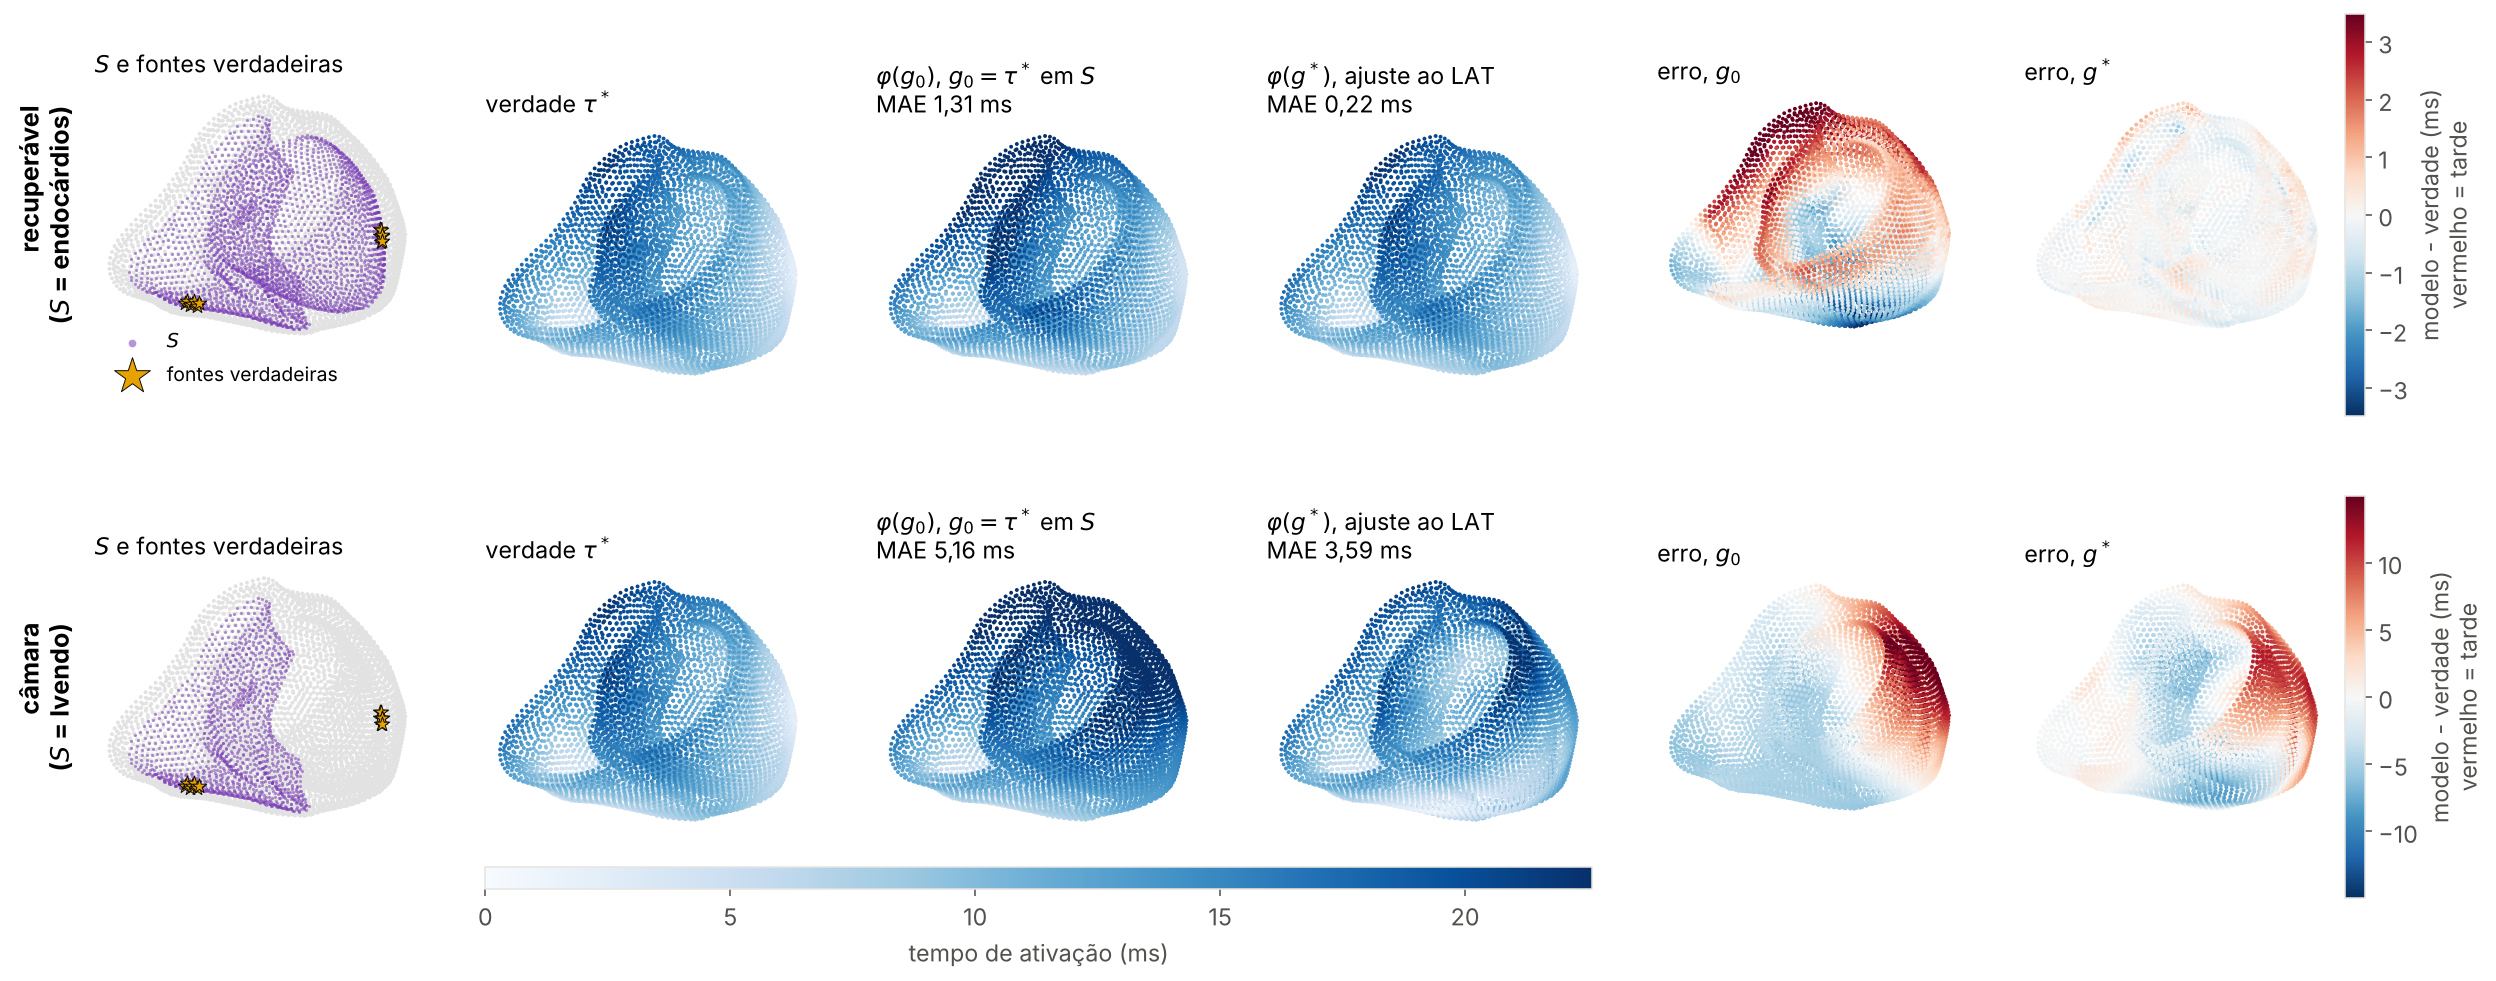
\includegraphics[width=\linewidth]{vent_mapas.png}\par
  {\scriptsize Roxo: $S$; estrelas: as fontes verdadeiras (no chamber, a do VD fica fora de $S$). Erro com as médias removidas.}
\end{frame}

\begin{frame}{Antes do inverso: ECG com $g$ dado}
  \centering
  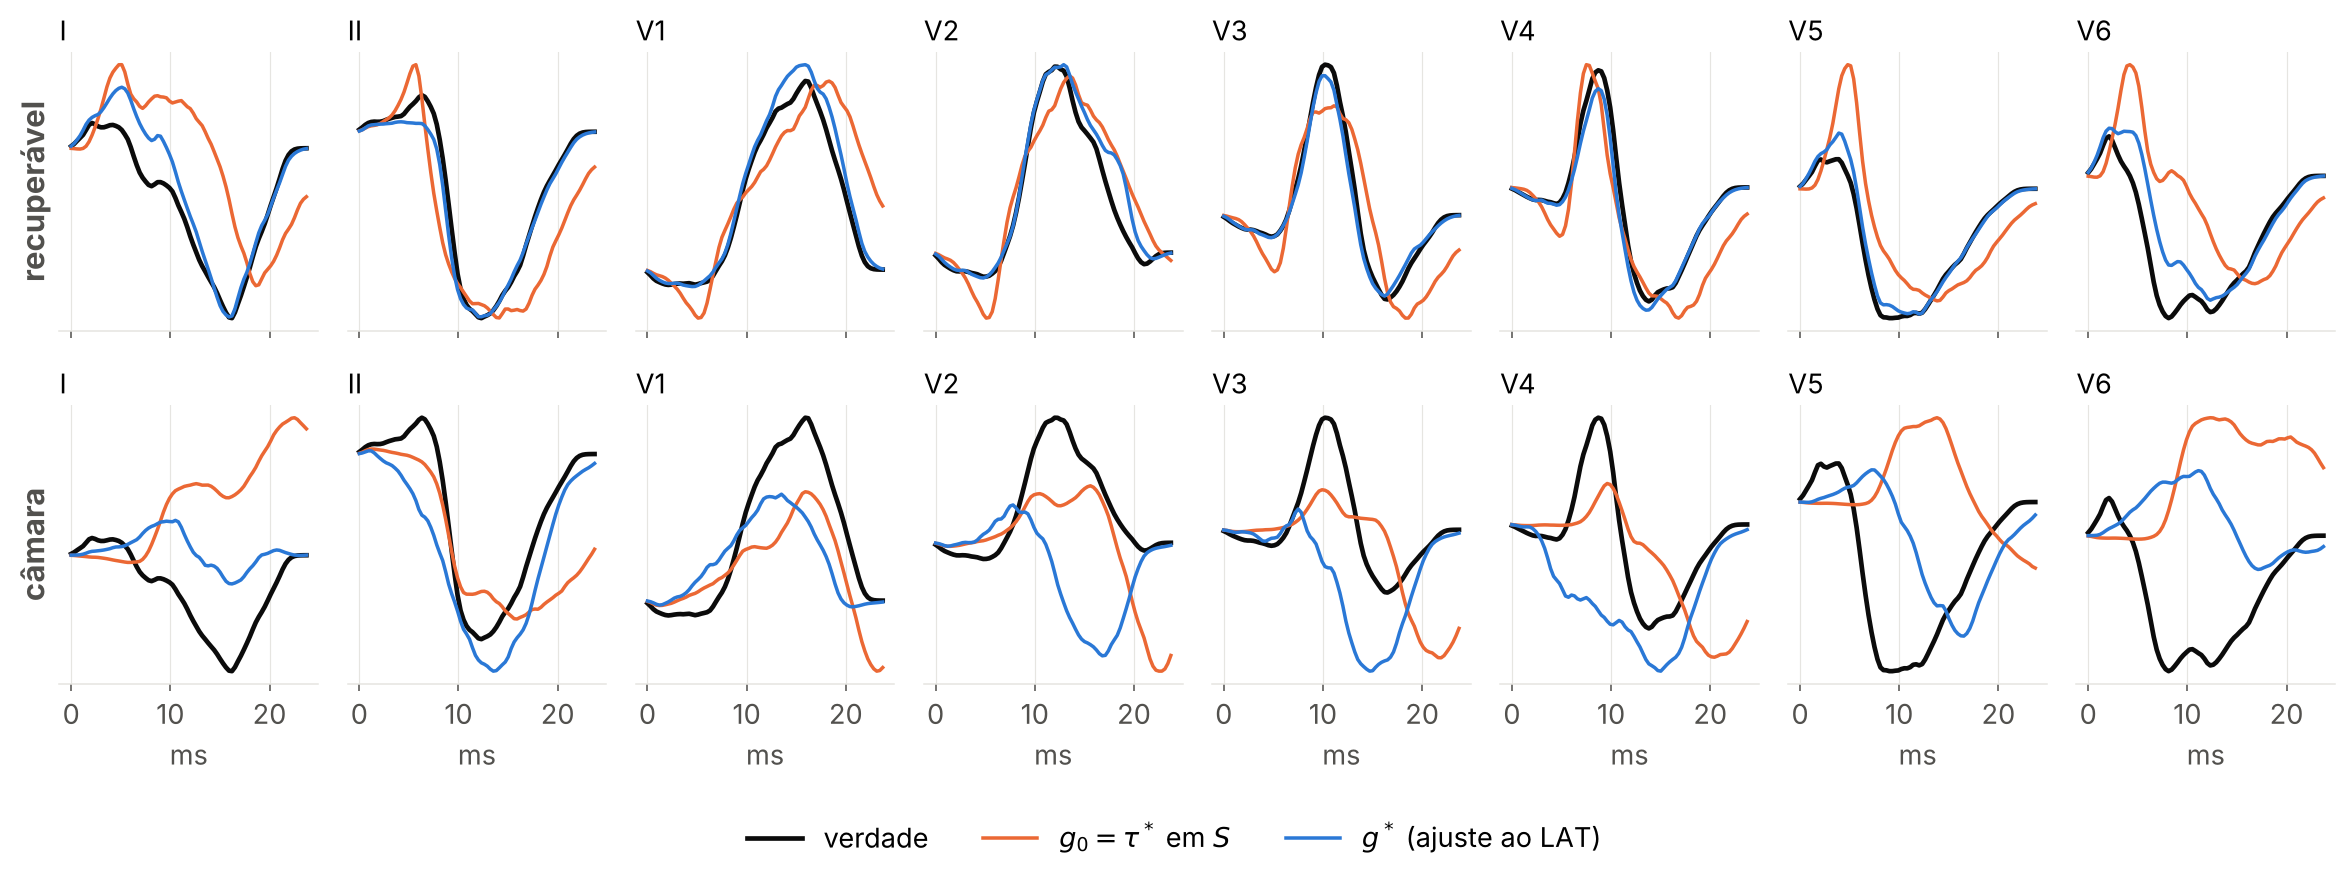
\includegraphics[width=\linewidth]{vent_ecg.png}\par
  {\small Erro relativo do ECG: recoverable $g_0$ 0,299, $g^*$ 0,032; chamber $g_0$ 1,282, $g^*$ 1,638.}
\end{frame}

\begin{frame}[label=tab_camara]{Inverso: chamber ($S$ = endocárdio do VE)}
  \centering
  \scriptsize
  \setlength{\tabcolsep}{5pt}
  \renewcommand{\arraystretch}{0.95}
  \begin{tabular}{@{}lcccccccc@{}}
    \toprule
    braço & ECG & corr & eik & $n$ & \shortstack{prof.\ 2ª\\(ms)} & \shortstack{$d_S$\\fonte 1} & \shortstack{$d_S$\\fonte 2} & \shortstack{$d_S$\\fonte 3}\\
    \midrule
    verdade & -- & -- & 0,231 & 2 & 8,9 & 0,00 & 0,50 & --\\
    sem $L_S$ & 0,010 & 0,57 & 0,172 & 1 & 0,0 & 0,43 {\tiny(8)} & 0,35 {\tiny(3)} & 0,03 {\tiny(2)}\\
    classic, $W=1$ & 0,034 & 0,72 & 0,223 & 2 & 3,5 & 0,01 {\tiny(8)} & 0,38 {\tiny(8)} & 0,00 {\tiny(3)}\\
    ring $k=1$, $W=1$ & 0,014 & 0,56 & 0,191 & 1 & 0,0 & 0,37 {\tiny(8)} & 0,46 {\tiny(3)} & 0,00 {\tiny(1)}\\
    ring $k=1$, $W=100$ & 0,038 & 0,48 & 0,237 & 1 & 0,0 & 0,27 {\tiny(8)} & 0,23 {\tiny(2)} & --\\
    floor, $W=1$ & 0,028 & 0,59 & 0,229 & 3 & 2,1 & 0,02 {\tiny(8)} & 0,40 {\tiny(7)} & 0,09 {\tiny(5)}\\
    floor, $W=100$ & 0,121 & 0,32 & 0,242 & 1 & 0,0 & 0,00 {\tiny(8)} & 0,00 {\tiny(3)} & 0,00 {\tiny(1)}\\
    \midrule
    \textbf{Método 1}, só ECG & 0,173 & 0,28 & 0,436 & 3 & 4,4 & 0,00 {\tiny(3)} & 0,00 {\tiny(3)} & 0,00 {\tiny(3)}\\
    \bottomrule
  \end{tabular}\par
  \medskip
  {\tiny ECG: erro relativo do ECG. corr: correlação com o mapa verdadeiro. eik: RMS de $\|\U\nabla\varphi\| - 1$.
  $n$: fontes com profundidade $\geq 1$ ms; prof.\ 2ª: profundidade da segunda fonte.
  $d_S$ fonte $k$: distância a $S$ da $k$-ésima fonte mais funda (entre parênteses, em quantas repetições ela aparece). Medianas sobre as repetições.}
\end{frame}

\begin{frame}[label=tab_recuperavel]{Inverso: recoverable ($S$ = endocárdios)}
  \centering
  \scriptsize
  \setlength{\tabcolsep}{3.7pt}
  \renewcommand{\arraystretch}{0.86}
  \begin{tabular}{@{}lccccccccc@{}}
    \toprule
    braço & rep. & ECG & corr & eik & $n$ & \shortstack{prof.\ 2ª\\(ms)} & \shortstack{$d_S$\\fonte 1} & \shortstack{$d_S$\\fonte 2} & \shortstack{$d_S$\\fonte 3}\\
    \midrule
    verdade &  & -- & -- & 0,231 & 2 & 8,9 & 0,00 & 0,00 & --\\
    sem $L_S$ & 8 & 0,010 & 0,57 & 0,172 & 1 & 0,0 & 0,00 {\tiny(8)} & 0,00 {\tiny(3)} & 0,03 {\tiny(2)}\\
    classic, $W=1$ & 8 & 0,010 & 0,53 & 0,174 & 1 & 0,0 & 0,00 {\tiny(8)} & 0,07 {\tiny(2)} & 0,00 {\tiny(1)}\\
    ring $k=1$, $W=1$ & 3 & 0,010 & 0,78 & 0,206 & 2 & 3,8 & 0,00 {\tiny(3)} & 0,01 {\tiny(2)} & 0,00 {\tiny(1)}\\
    ring $k=1$, $W=10$ & 3 & 0,016 & 0,53 & 0,220 & 1 & 0,0 & 0,02 {\tiny(3)} & 0,00 {\tiny(1)} & 0,00 {\tiny(1)}\\
    ring $k=1$, $W=100$ & 3 & 0,103 & 0,20 & 0,232 & 1 & 0,0 & 0,05 {\tiny(3)} & -- & --\\
    ring $k=3$, $W=1$ & 3 & 0,010 & 0,52 & 0,171 & 1 & 0,0 & 0,00 {\tiny(3)} & -- & --\\
    ring $k=3$, $W=10$ & 3 & 0,022 & 0,52 & 0,208 & 1 & 0,0 & 0,00 {\tiny(3)} & 0,08 {\tiny(1)} & --\\
    ring $k=3$, $W=100$ & 3 & 0,055 & 0,69 & 0,333 & 2 & 2,7 & 0,04 {\tiny(3)} & 0,00 {\tiny(2)} & 0,00 {\tiny(1)}\\
    ring $k=6$, $W=1$ & 3 & 0,060 & 0,29 & 0,306 & 2 & 1,3 & 0,07 {\tiny(3)} & 0,00 {\tiny(2)} & --\\
    ring $k=6$, $W=10$ & 3 & 0,148 & $-$0,04 & 0,428 & 1 & 0,0 & 0,06 {\tiny(3)} & -- & --\\
    ring $k=6$, $W=100$ & 3 & 0,250 & 0,33 & 0,274 & 1 & 0,0 & 0,06 {\tiny(3)} & -- & --\\
    floor, $W=1$ & 8 & 0,010 & 0,60 & 0,169 & 1 & 0,0 & 0,00 {\tiny(8)} & 0,00 {\tiny(3)} & --\\
    floor, $W=10$ & 8 & 0,013 & 0,52 & 0,165 & 1 & 0,0 & 0,00 {\tiny(8)} & 0,00 {\tiny(1)} & --\\
    floor, $W=100$ & 8 & 0,022 & 0,61 & 0,165 & 1 & 0,0 & 0,00 {\tiny(8)} & 0,00 {\tiny(2)} & --\\
    \midrule
    \textbf{Método 1}, só LAT & 3 & 0,027 & 1,00 & 0,194 & 2 & 8,6 & 0,00 {\tiny(3)} & 0,00 {\tiny(3)} & --\\
    \textbf{Método 1}, só ECG & 3 & 0,002 & 0,81 & 0,236 & 5 & 5,8 & 0,00 {\tiny(3)} & 0,00 {\tiny(3)} & 0,00 {\tiny(3)}\\
    \bottomrule
  \end{tabular}\par
  \medskip
  {\tiny Colunas como na página anterior; rep.: número de repetições.}
\end{frame}

% Parte 4: resultados de 15/10 em DTI004 truth5ti_s1 (Metodo 1).
% Codigo: tools/camps_gstar/ no repo bolsaic -> problems/camps_dti004/ no MMC:
% fit_g.py (g*), train_lat_then_ecg.py (inicios A e B, ECG), train_noise_sweep.py,
% train_known_g.py. Figuras e linhas das tabelas: scripts/deck_figs.py.
% So os otimizadores mantidos apos a varredura (Adam 1e-4 e 5e-4).

\section{Começar do LAT (DTI004)}

\begin{frame}{O teste: um início que já reproduz o LAT}
  \small
  \begin{itemize}\setlength{\itemsep}{0.25em}
    \item Verdade: DTI004, 5 raízes em $t = 0$ entre os 601 candidatos de Camps; transversalmente isotrópica (0,065 / 0,050 cm/ms), sem camada rápida; LAT por FIM, ECG pelo campo de chumbo (8 derivações).
    \item $g_0$: o LAT verdadeiro restrito a $S$.
    \item $g^*$: o $g$ livre em $S$ (601 números) que minimiza o erro de LAT do Método 1, partindo de $g_0$; para em $3{,}0 \cdot 10^{-5}$ com qualquer passo.
    \item \textbf{Início A}: a rede treinada no LAT, a partir de pesos aleatórios (5000 passos).
    \item \textbf{Início B}: a rede ajustada a $g^*$ (regressão em $g$).
    \item Depois, o inverso só com o ECG: 1000 iterações, Adam com passo em cosseno; velocidades a $\pm 1\%$ da verdade, $H_\varepsilon$ congelado.
  \end{itemize}
\end{frame}

\begin{frame}{Início A $\times$ início B}
  \centering
  \scriptsize
  \setlength{\tabcolsep}{3.4pt}
  \renewcommand{\arraystretch}{1.15}
  \begin{tabular}{@{}lcccc@{\hspace{1em}}cccc@{}}
    \toprule
    & \multicolumn{4}{c}{A: rede treinada no LAT} & \multicolumn{4}{c}{B: rede ajustada a $g^*$}\\
    \cmidrule(r{1em}){2-5}\cmidrule{6-9}
    estágio & \shortstack{LAT rms\\(ms)} & \shortstack{LAT MAE\\(ms)} & corr & ECG & \shortstack{LAT rms\\(ms)} & \shortstack{LAT MAE\\(ms)} & corr & ECG\\
    \midrule
\inputrows{sections/tab_hoje.tex}
    \bottomrule
  \end{tabular}\par
  \medskip
  {\tiny Verdade truth5ti\_s1. $g_0$ e $g^*$ são referências (mesmos valores nas duas colunas).
  ECG: erro relativo do ECG. Uma rodada por linha; a rede de início é a mesma (bit a bit) nas duas linhas do inverso.}
\end{frame}

\begin{frame}{Mapas de ativação em cada estágio}
  \centering
  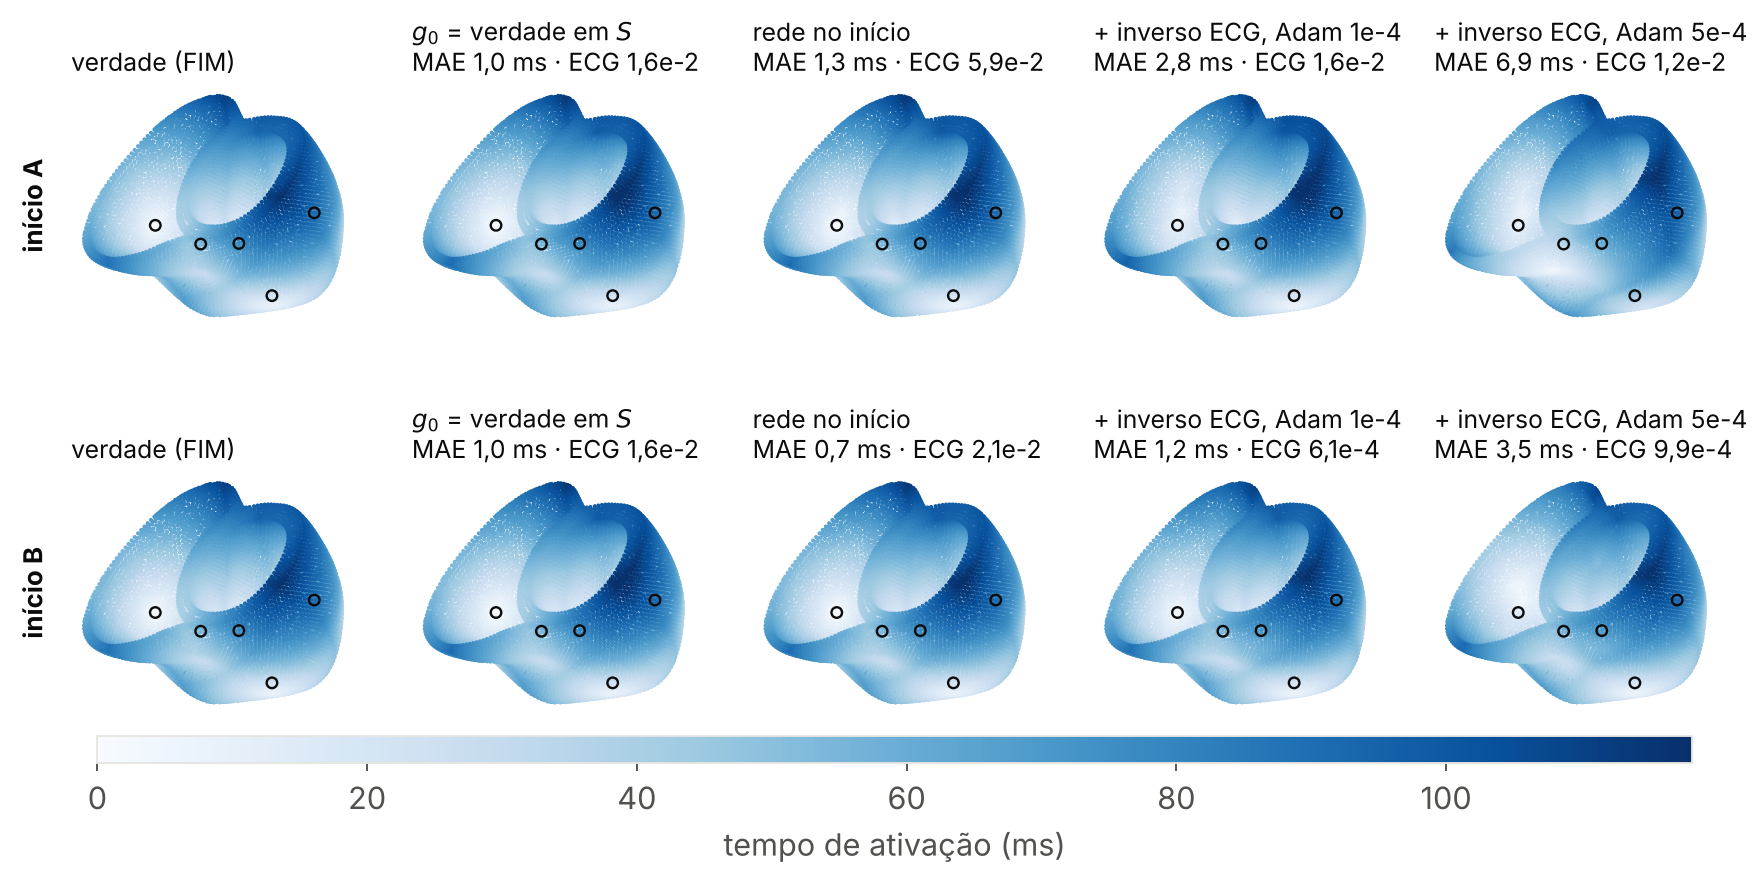
\includegraphics[width=0.97\linewidth]{hoje_mapas.png}
\end{frame}

\begin{frame}{Erro de LAT em cada estágio}
  \centering
  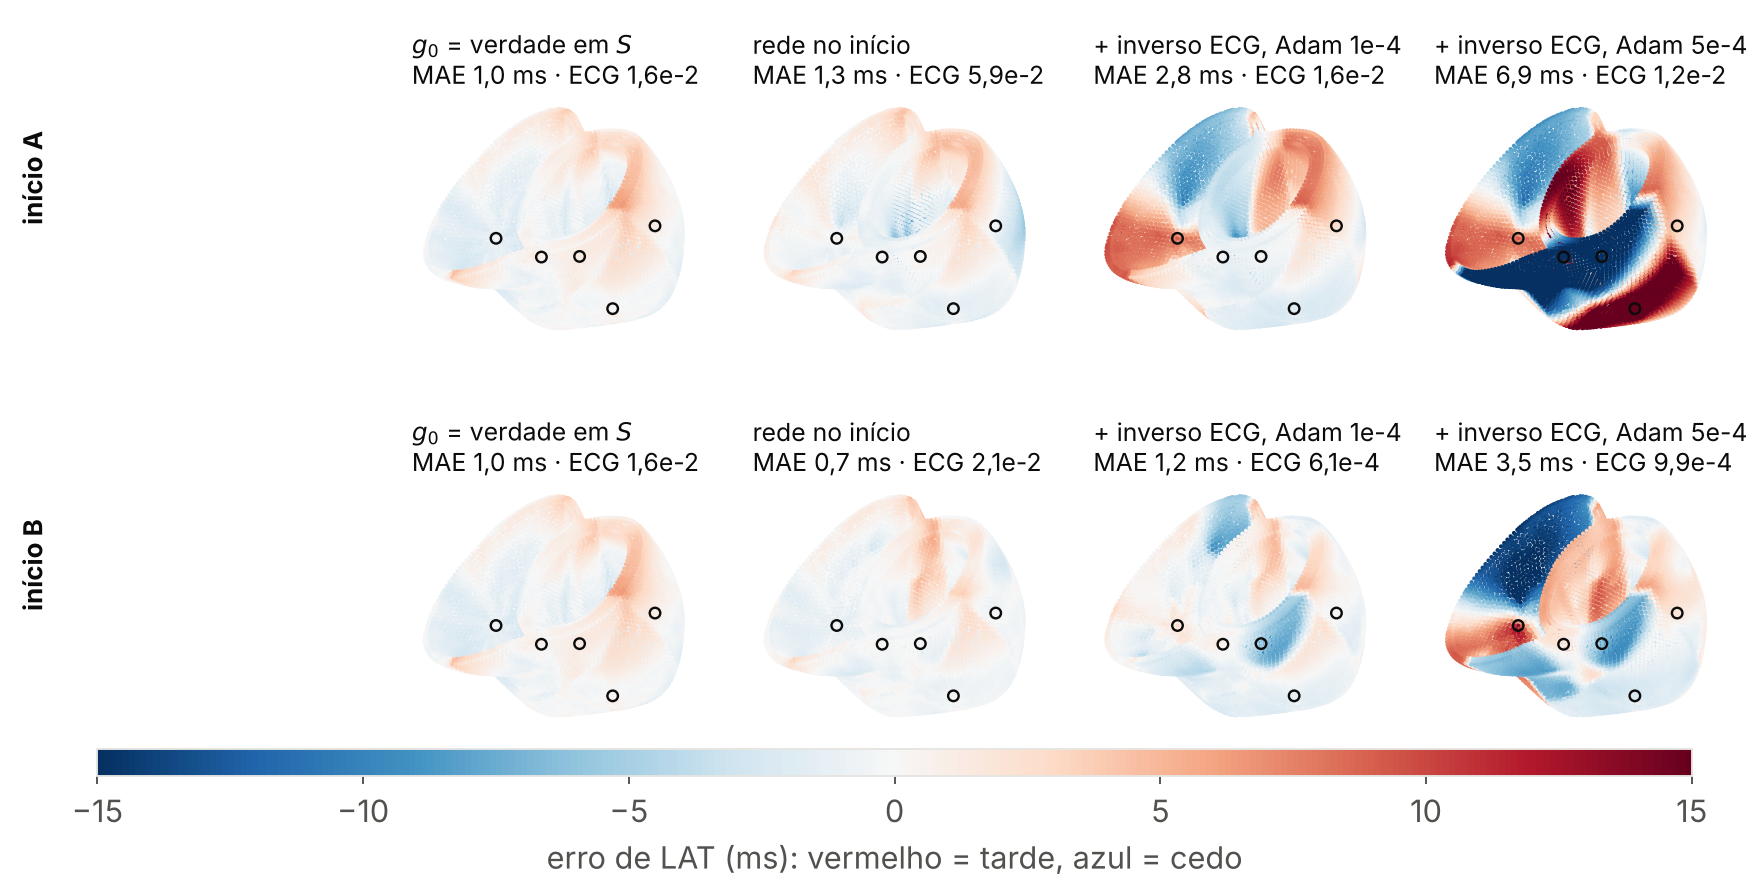
\includegraphics[width=0.97\linewidth]{hoje_erro.png}
\end{frame}

\begin{frame}{Sensibilidade ao ponto de partida}
  \centering
  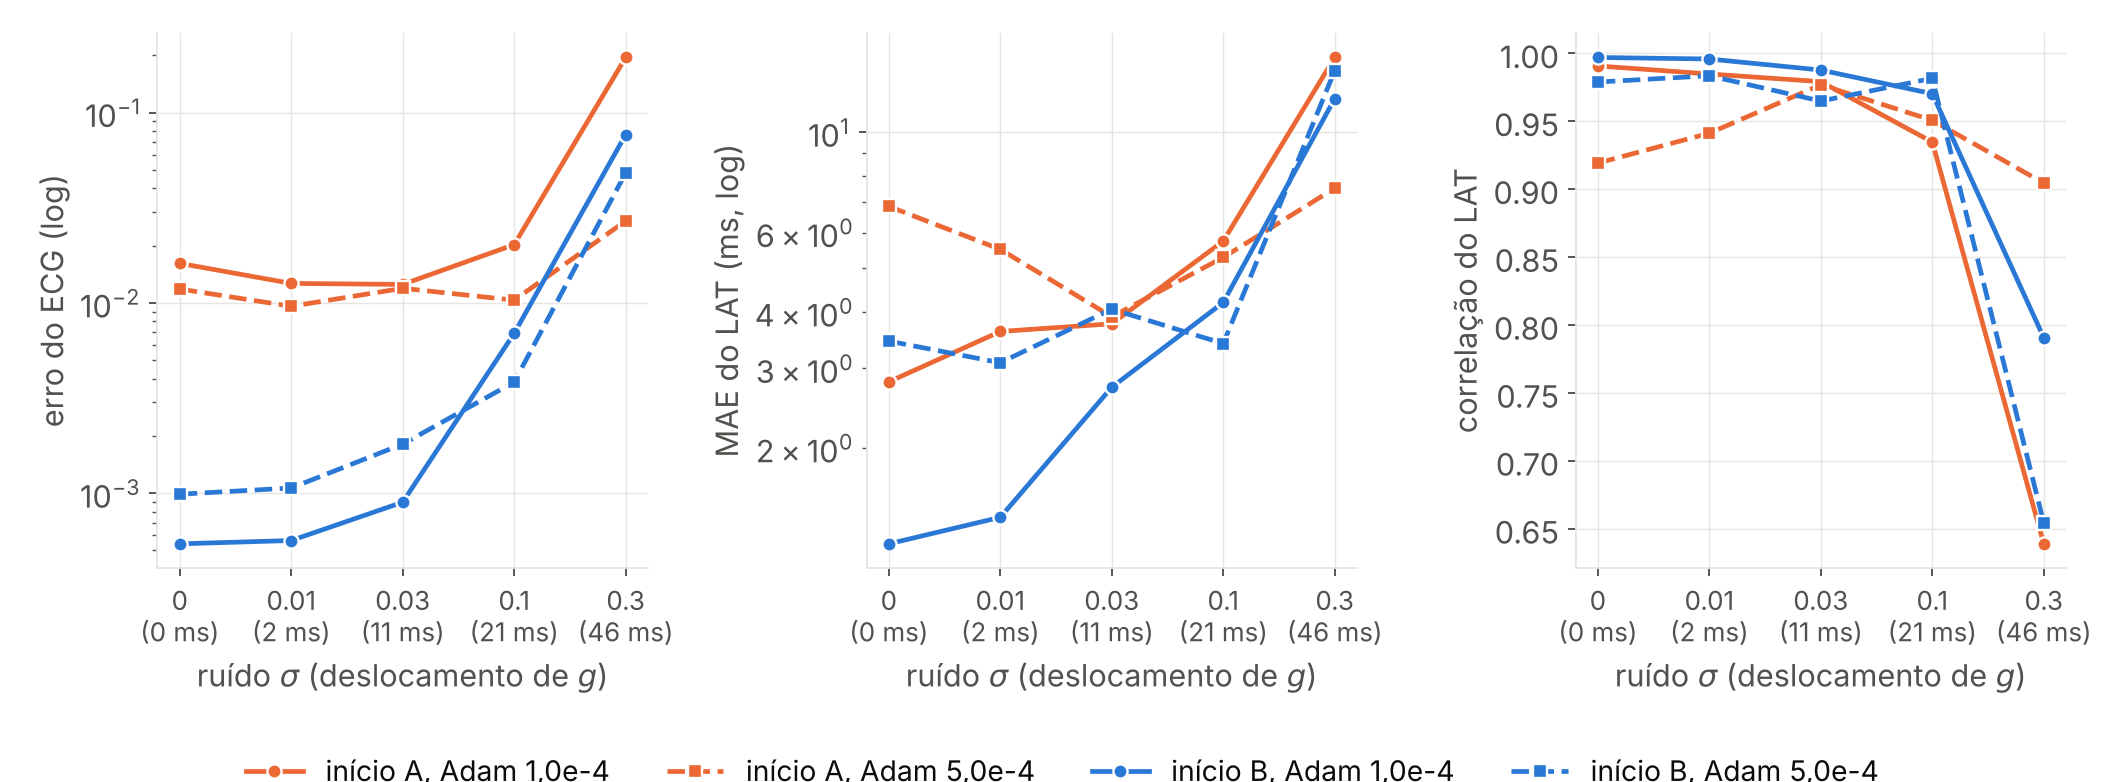
\includegraphics[width=\linewidth]{hoje_ruido.png}\par
  \smallskip
  {\scriptsize Ruído nos pesos da rede de início: $\sigma \times$ desvio de cada tensor; o mesmo ruído em A e B.
  Entre parênteses, quanto o ruído desloca $g$ nos candidatos dominantes. Mediana de 3 sorteios (1 em $\sigma = 0$).}
\end{frame}

\begin{frame}{Teste com $g$ conhecido: o alvo gerado pelo próprio Método 1}
  \centering
  \scriptsize
  \setlength{\tabcolsep}{4.5pt}
  \renewcommand{\arraystretch}{1.1}
  \begin{tabular}{@{}lcccccc@{}}
    \toprule
    início & \shortstack{ECG\\início} & \shortstack{ECG\\fim} & \shortstack{corr\\fim} & \shortstack{LAT MAE\\fim (ms)} & \shortstack{rms de $g$\\início (ms)} & \shortstack{rms de $g$\\fim (ms)}\\
    \midrule
\inputrows{sections/tab_gconhecido.tex}
    \bottomrule
  \end{tabular}\par
  \medskip
  {\tiny $g_{\mathrm{v}}$: o LAT verdadeiro em $S$; o mapa e o ECG alvo saem do Método 1 com $g_{\mathrm{v}}$ (erro zero é atingível).
  Ruído direto em $g$ (ms). Inverso só com ECG, Adam $5 \cdot 10^{-4}$, 1000 iterações.
  rms de $g$: nos 21 candidatos com $g_{\mathrm{v}} - \min < 10$ ms. Uma rodada por linha.}
\end{frame}

% Parte 5: DTI004, recuperacao completa, Metodo 1 x Camps.
% problems/camps_dti004/outputs/set1/SUMMARY.md e truth5ti_s*_{m1,camps}.json
% (2026-10-13); tabela e figura: scripts/deck_figs.py.

\section{DTI004: recuperação completa}

\begin{frame}{DTI004: Método 1 $\times$ Camps}
  \small
  \begin{itemize}\setlength{\itemsep}{0.3em}
    \item Seis verdades, cada uma com 5 root nodes em $t = 0$ entre os 601 candidatos de Camps; velocidades a $\pm 1\%$ da verdade nos dois métodos.
    \item \textbf{Camps}: SMC-ABC, 512 partículas; mapas por Dijkstra, discrepância de ECG por DTW; 16 núcleos de CPU.
    \item \textbf{Método 1}: 100 inicializações $\times$ 1000 iterações; mapas por FIM, ECG por lead field; uma GPU.
    \item Cada método contra a sua própria verdade (Dijkstra $\times$ FIM). O erro de ECG é a nossa métrica, não a que Camps otimiza.
  \end{itemize}
\end{frame}

\begin{frame}{Resultados por verdade}
  \centering
  \tiny
  \setlength{\tabcolsep}{3.6pt}
  \renewcommand{\arraystretch}{0.92}
  \begin{tabular}{@{}llcccccccccc@{}}
    \toprule
    verdade & método & soluções & \shortstack{tempo\\(min)} & corr & \shortstack{LAT MAE\\(ms)} & ECG & \shortstack{root\\nodes} & \shortstack{verdade $\to$\\recup.\ (cm)} & \shortstack{recup.\ $\to$\\verdade (cm)} & \shortstack{$\geq 2$ roots\\a $\leq 1$ cm}\\
    \midrule
\inputrows{sections/tab_dti004.tex}
    \bottomrule
  \end{tabular}\par
  \medskip
  {\tiny Medianas sobre as soluções (partículas ou inicializações). verdade $\to$ recup.: média, sobre os 5 root nodes verdadeiros, da distância geodésica ao recuperado mais próximo;
  recup.\ $\to$ verdade: o inverso. Root nodes: candidatos ativos (Camps); fontes com profundidade $\geq 1$ ms (Método 1).
  Última coluna: fração das soluções com ao menos 2 root nodes verdadeiros a até 1 cm.}
\end{frame}

\begin{frame}{Todas as soluções das seis verdades}
  \centering
  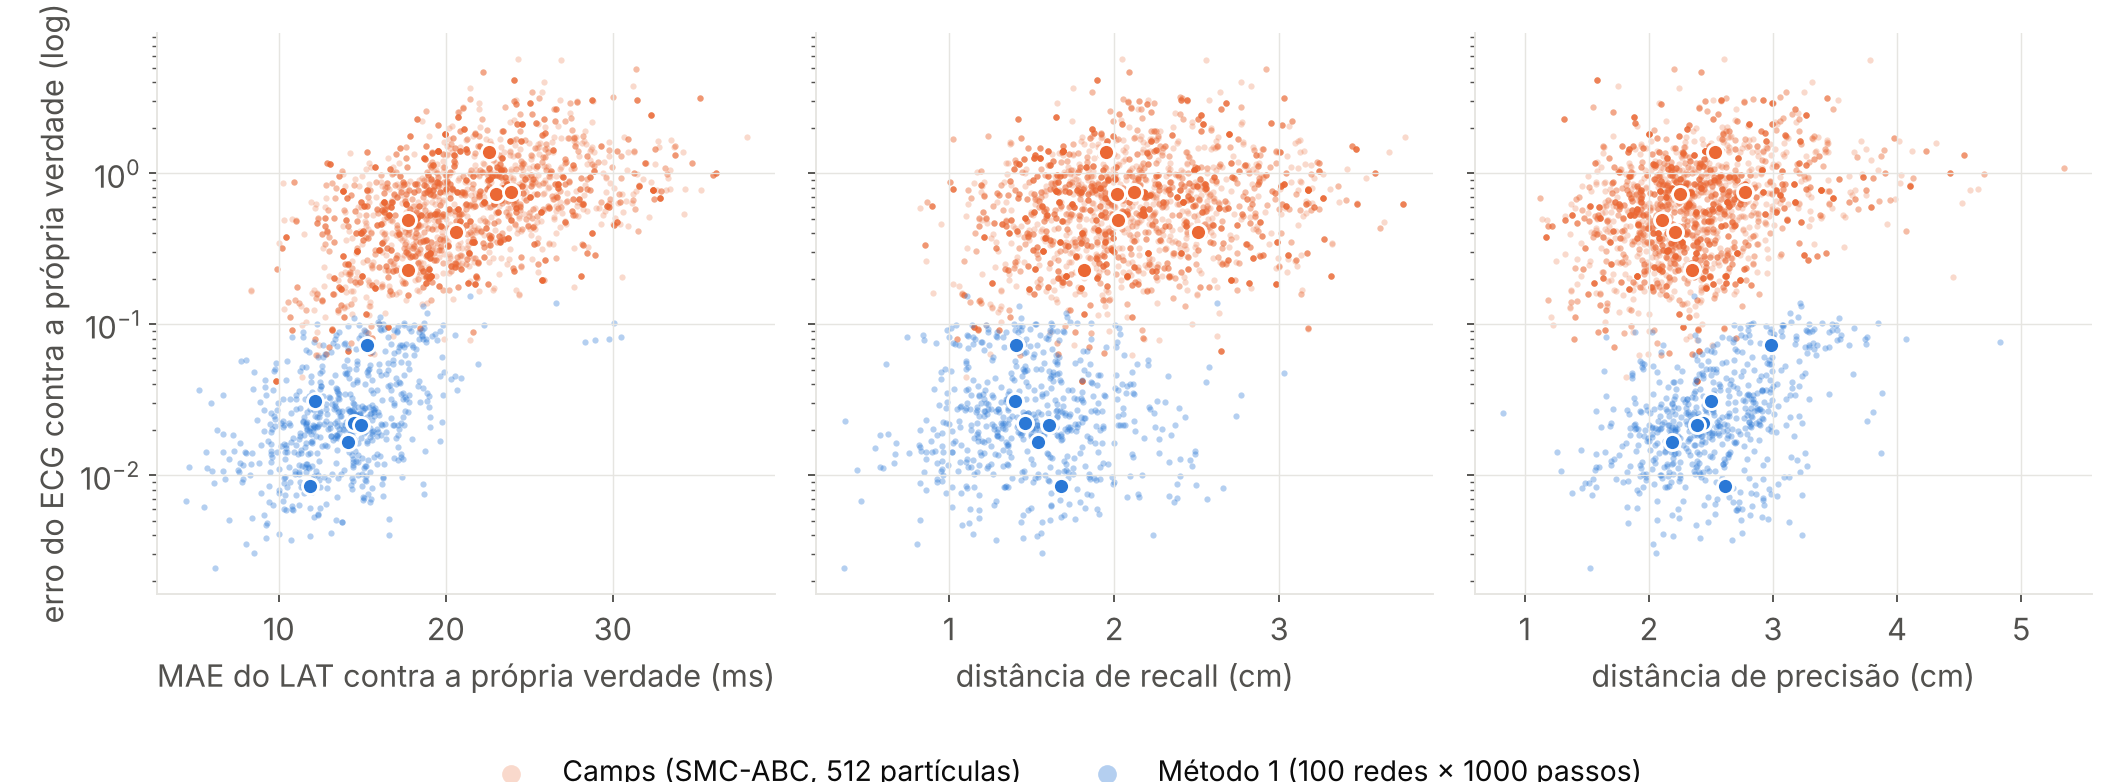
\includegraphics[width=\linewidth]{dti004_membros.png}\par
  \smallskip
  {\scriptsize Pontos: cada solução; círculos grandes: a mediana de cada verdade.}
\end{frame}


\end{document}
